
\usetikzlibrary{arrows}
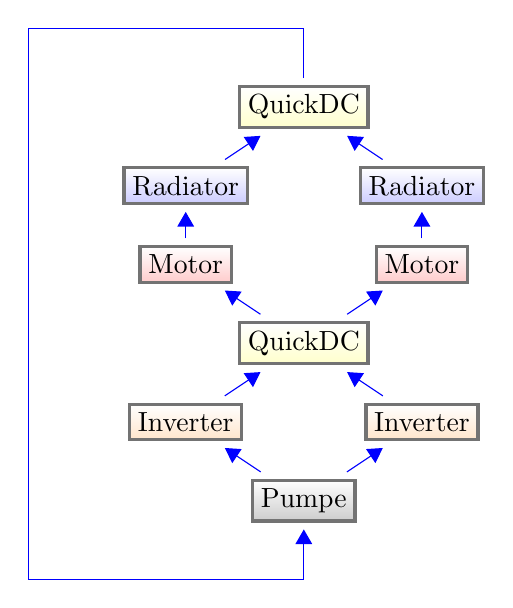
\begin{tikzpicture}
\tikzstyle{radiator} = [draw,outer sep=3,inner sep=3,line width=1, very thick, draw=black!55, top color=white,bottom color=blue!20]
\tikzstyle{Pumpe} = [draw,outer sep=3,inner sep=3,line width=1, very thick, draw=black!55, top color=white,bottom color=black!20]
\tikzstyle{Inverter} = [draw,outer sep=3,inner sep=3,line width=1, very thick, draw=black!55, top color=white,bottom color=orange!20]
\tikzstyle{Motor} = [draw,outer sep=3,inner sep=3,line width=1, very thick, draw=black!55, top color=white,bottom color=red!20]
\tikzstyle{Quickconnect} = [draw,outer sep=3,inner sep=3,line width=1, very thick, draw=black!55, top color=white,bottom color=yellow!20]

\node [radiator] (v7) at (-2,-2.5) {Radiator};
\node [radiator] (v8) at (1,-2.5) {Radiator};
\node [Pumpe] (v1) at (-0.5,-6.5) {Pumpe};
\node [Inverter] (v2) at (-2,-5.5) {Inverter};
\node [Inverter] (v3) at (1,-5.5) {Inverter};
\node [Motor] (v6) at (-2,-3.5) {Motor};
\node [Motor] (v5) at (1,-3.5) {Motor};
\node [Quickconnect] (v4) at (-0.5,-4.5) {QuickDC};
\node [Quickconnect] (v9) at (-0.5,-1.5) {QuickDC};

\tikzstyle{Leitungen} = [-triangle 60, color=blue]
\draw [Leitungen] (v1) edge (v2);
\draw [Leitungen] (v1) edge (v3);
\draw [Leitungen] (v2) edge (v4);
\draw [Leitungen] (v3) edge (v4);
\draw [Leitungen] (v4) edge (v5);
\draw [Leitungen] (v4) edge (v6);
\draw [Leitungen] (v6) edge (v7);
\draw [Leitungen] (v5) edge (v8);
\draw [Leitungen] (v7) edge (v9);
\draw [Leitungen] (v8) edge (v9);

\draw [Leitungen] (v9) -- (-0.5,-0.5) -- (-4,-0.5) -- (-4,-7.5) -- (-0.5,-7.5) -- (v1);
\end{tikzpicture}